\section{Scope, interpretation, and evidence}
\label{sec:scope}
The source article \emph{Euclidean geometry} names congruence, triangle
angle sums, the Pythagorean theorem, Thales' theorem, Ptolemy's theorem,
Platonic solids, and scaling of area and volume. Its relevant outgoing
links include Euclid's \emph{Elements}, circles, straightedge-and-compass
construction, analytic geometry, the parallel postulate, Heron's formula,
Ceva's theorem, Menelaus' theorem, the angle-bisector theorem, the
nine-point circle, and the butterfly theorem \cite{wiki}.
This report develops a substantial collection from that neighborhood.
We give individual proofs rather than treating a general decision procedure
as a substitute for an explanation of the geometry.

The main mathematical choice is to interpret exact points by pairs of
finite real-algebraic records. This gives an actual arithmetic interpretation,
not an assertion that a proof about Lean's ambient real numbers is thereby
a proof in iPRA. Polynomial identities already make sense over rational
coordinates. Square roots and exact intersection constructions require a
larger coded domain. Sections~\ref{sec:foundation}--\ref{sec:elimination}
construct it and explain its relation to the ordinary real plane.

\paragraph{Three different statements.}
For a geometric formula $\phi$, the assertion that $\phi$ is true over
$\R^2$, a proof of $\phi$ in Lean's metatheory, and a derivation of
$\phi^\#$ in iPRA are different achievements. Here $\phi^\#$ replaces
points, lines, scalar operations, and quantified geometric objects by the
specific numerical codes below. Our human arguments prove these translated
statements using defining equations, decidable arithmetic, and
quantifier-free induction. The supplied Lean work targets the final,
object-theory assertion explicitly, but its complete formalization remains
work to do. All source and verification files state that boundary.

\paragraph{Reuse and provenance.}
ProveIt was inspected at commit
\nolinkurl{bbb85238dac533fc4b7b84a750cca864fe35fed5}.
Its \texttt{PrimitiveRecursiveArithmetic/README.md} distinguishes the
\texttt{ConciseIPRA}, \texttt{Derivations}, and \texttt{Bridge} libraries
from delivered research packets. In particular it warns that the packet
collection itself is not uniformly verified. We use the actual source
interfaces of \nolinkurl{Core/Tactic.lean}, \nolinkurl{Core/IntCertificates.lean},
\nolinkurl{Geometry/TriangleFormulas.lean}, and
\nolinkurl{Geometry/PlatonicSolids.lean}; these are not replaced by conjectural
API names. The earlier packet
\nolinkurl{planar_euclidean_geometry_ipra_2026-11-20} supplies a useful
bounded algebraic-field and elimination architecture. We rederive the
needed arguments below, and do not present that architecture, Heron's
identity, or the five-symbol counting argument as new discoveries
\cite{proveit,planar,trianglecore,platoniccore}.

\paragraph{What the scope does not silently assume.}
All divisions have a displayed nonzero denominator. Strict inequalities
on coded algebraic numbers are decidable; no decision rule for equality of
arbitrary computable real names is used. A positive square root is selected
by its sign, not by an ambiguous algebraic equation. Statements about a
simple polygon require an orientation/triangulation certificate, and
statements about a spherical polyhedral surface require a finite
cellulation certificate. Arbitrary compact sets, unrestricted completeness,
all higher-dimensional regular polytopes, and the transcendence of $\pi$
are not claimed as consequences of the elementary coordinate arguments.

\paragraph{How to read the report.}
Readers interested first in geometry can start with
Section~\ref{sec:affine}, using $\K$ as an exact ordered field with square
roots of nonnegative elements. The foundation then explains why this
notation abbreviates arithmetic. The final inventory records each proved
result, its source neighborhood, and its representation. Several theorems
contain multiple familiar consequences; the inventory counts each labeled
result once, rather than inflating the total by counting every equation.
\begin{figure}[htbp]
\centering
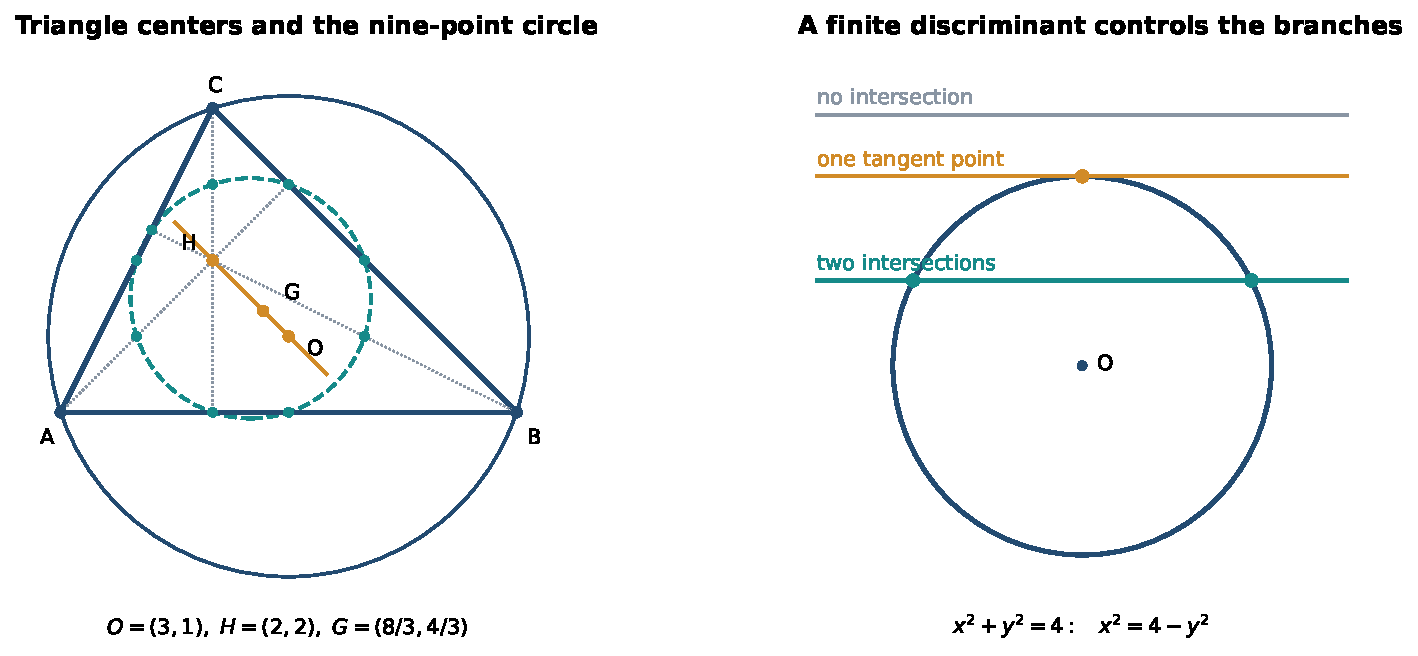
\includegraphics[width=\textwidth]{figures/centers-and-intersections.pdf}
\caption{Two themes of the portfolio. Left: explicit triangle-center
coordinates give the Euler line and nine-point circle. Right: the sign
of one algebraic discriminant gives the complete line--circle intersection
classification. The drawings illustrate the exact proofs; they are not
used as evidence for them.}
\end{figure}
